\section{予測モデルと精度検証}
% \paragraph{来訪・帰宅記録の取得}
来訪・帰宅時刻のみを対象とし在室予測を行うため，入退室記録から各ユーザの当日における最初の入室時刻と最後の退室時刻のみを取得する．
日を跨いだ滞在や退室記録の欠損といった例外的なケースには「退室なし」として前処理が施されている．
また，微小な差異が過度な影響を与えてしまうのを防ぐため，30分単位に丸めて処理されている．


% \paragraph{来訪・帰宅記録のクラスタリングを用いた特徴量の抽出}
ユーザは曜日ごとに複数の異なる行動パターンを示す可能性があるため，各曜日について複数クラスタを前提とした分析が行われている．
このシステムではガウス混合モデルをクラスタリング手法として採用し，上限を設定した上でベイズ情報量基準が最も小さくなるクラスタ数を採用している．
図\ref{fig:prediction}(\subref{fig:befClus})をクラスタリングすると\ref{fig:prediction}(\subref{fig:aftClus})のように三つのクラスタに分類される．
% この構成により，データの分布に柔軟に対応しつつ過学習を避けながら最適なクラスタ数を自動で決定できる．
この処理で得られた複数のクラスタをそれぞれ1つの正規分布とみなし，期間における各クラスタに属するデータ数の割合を元に重みを定義している．
各正規分布を累積分布関数に変換結果を図\ref{fig:prediction}(\subref{fig:befWeig})に示し，重みを反映させた累積分布関数は図\ref{fig:prediction}(\subref{fig:aftWeig})のようになる．
この構成により，曜日ごとの来訪頻度も確率推定に反映されている．


% \paragraph{ユーザ行動の発生予測時刻}
このシステムでは「任意の時刻を基準としたユーザ行動の発生確率」と「ユーザ行動の発生予測時刻」を導出している．
任意の時刻を基準としたユーザ行動の発生確率は，各クラスタの累積分布関数に対応する重みをかけて合算したものとしている．
図\ref{fig:prediction}(\subref{fig:aftWeig})の場合は図\ref{fig:prediction}(\subref{fig:synth})のようなグラフとなる．
ユーザ行動の発生予測時刻は，各クラスタの平均時刻に対応する重みをかけて合算し，加重平均としている．
これにより，来訪確率の高低に関わらず，その日に最も高い確率で来訪すると見込まれる時刻が算出できる．

\begin{figure}[htb]
  \centering
  \subcaptionbox{クラスタリング前\label{fig:befClus}}{
    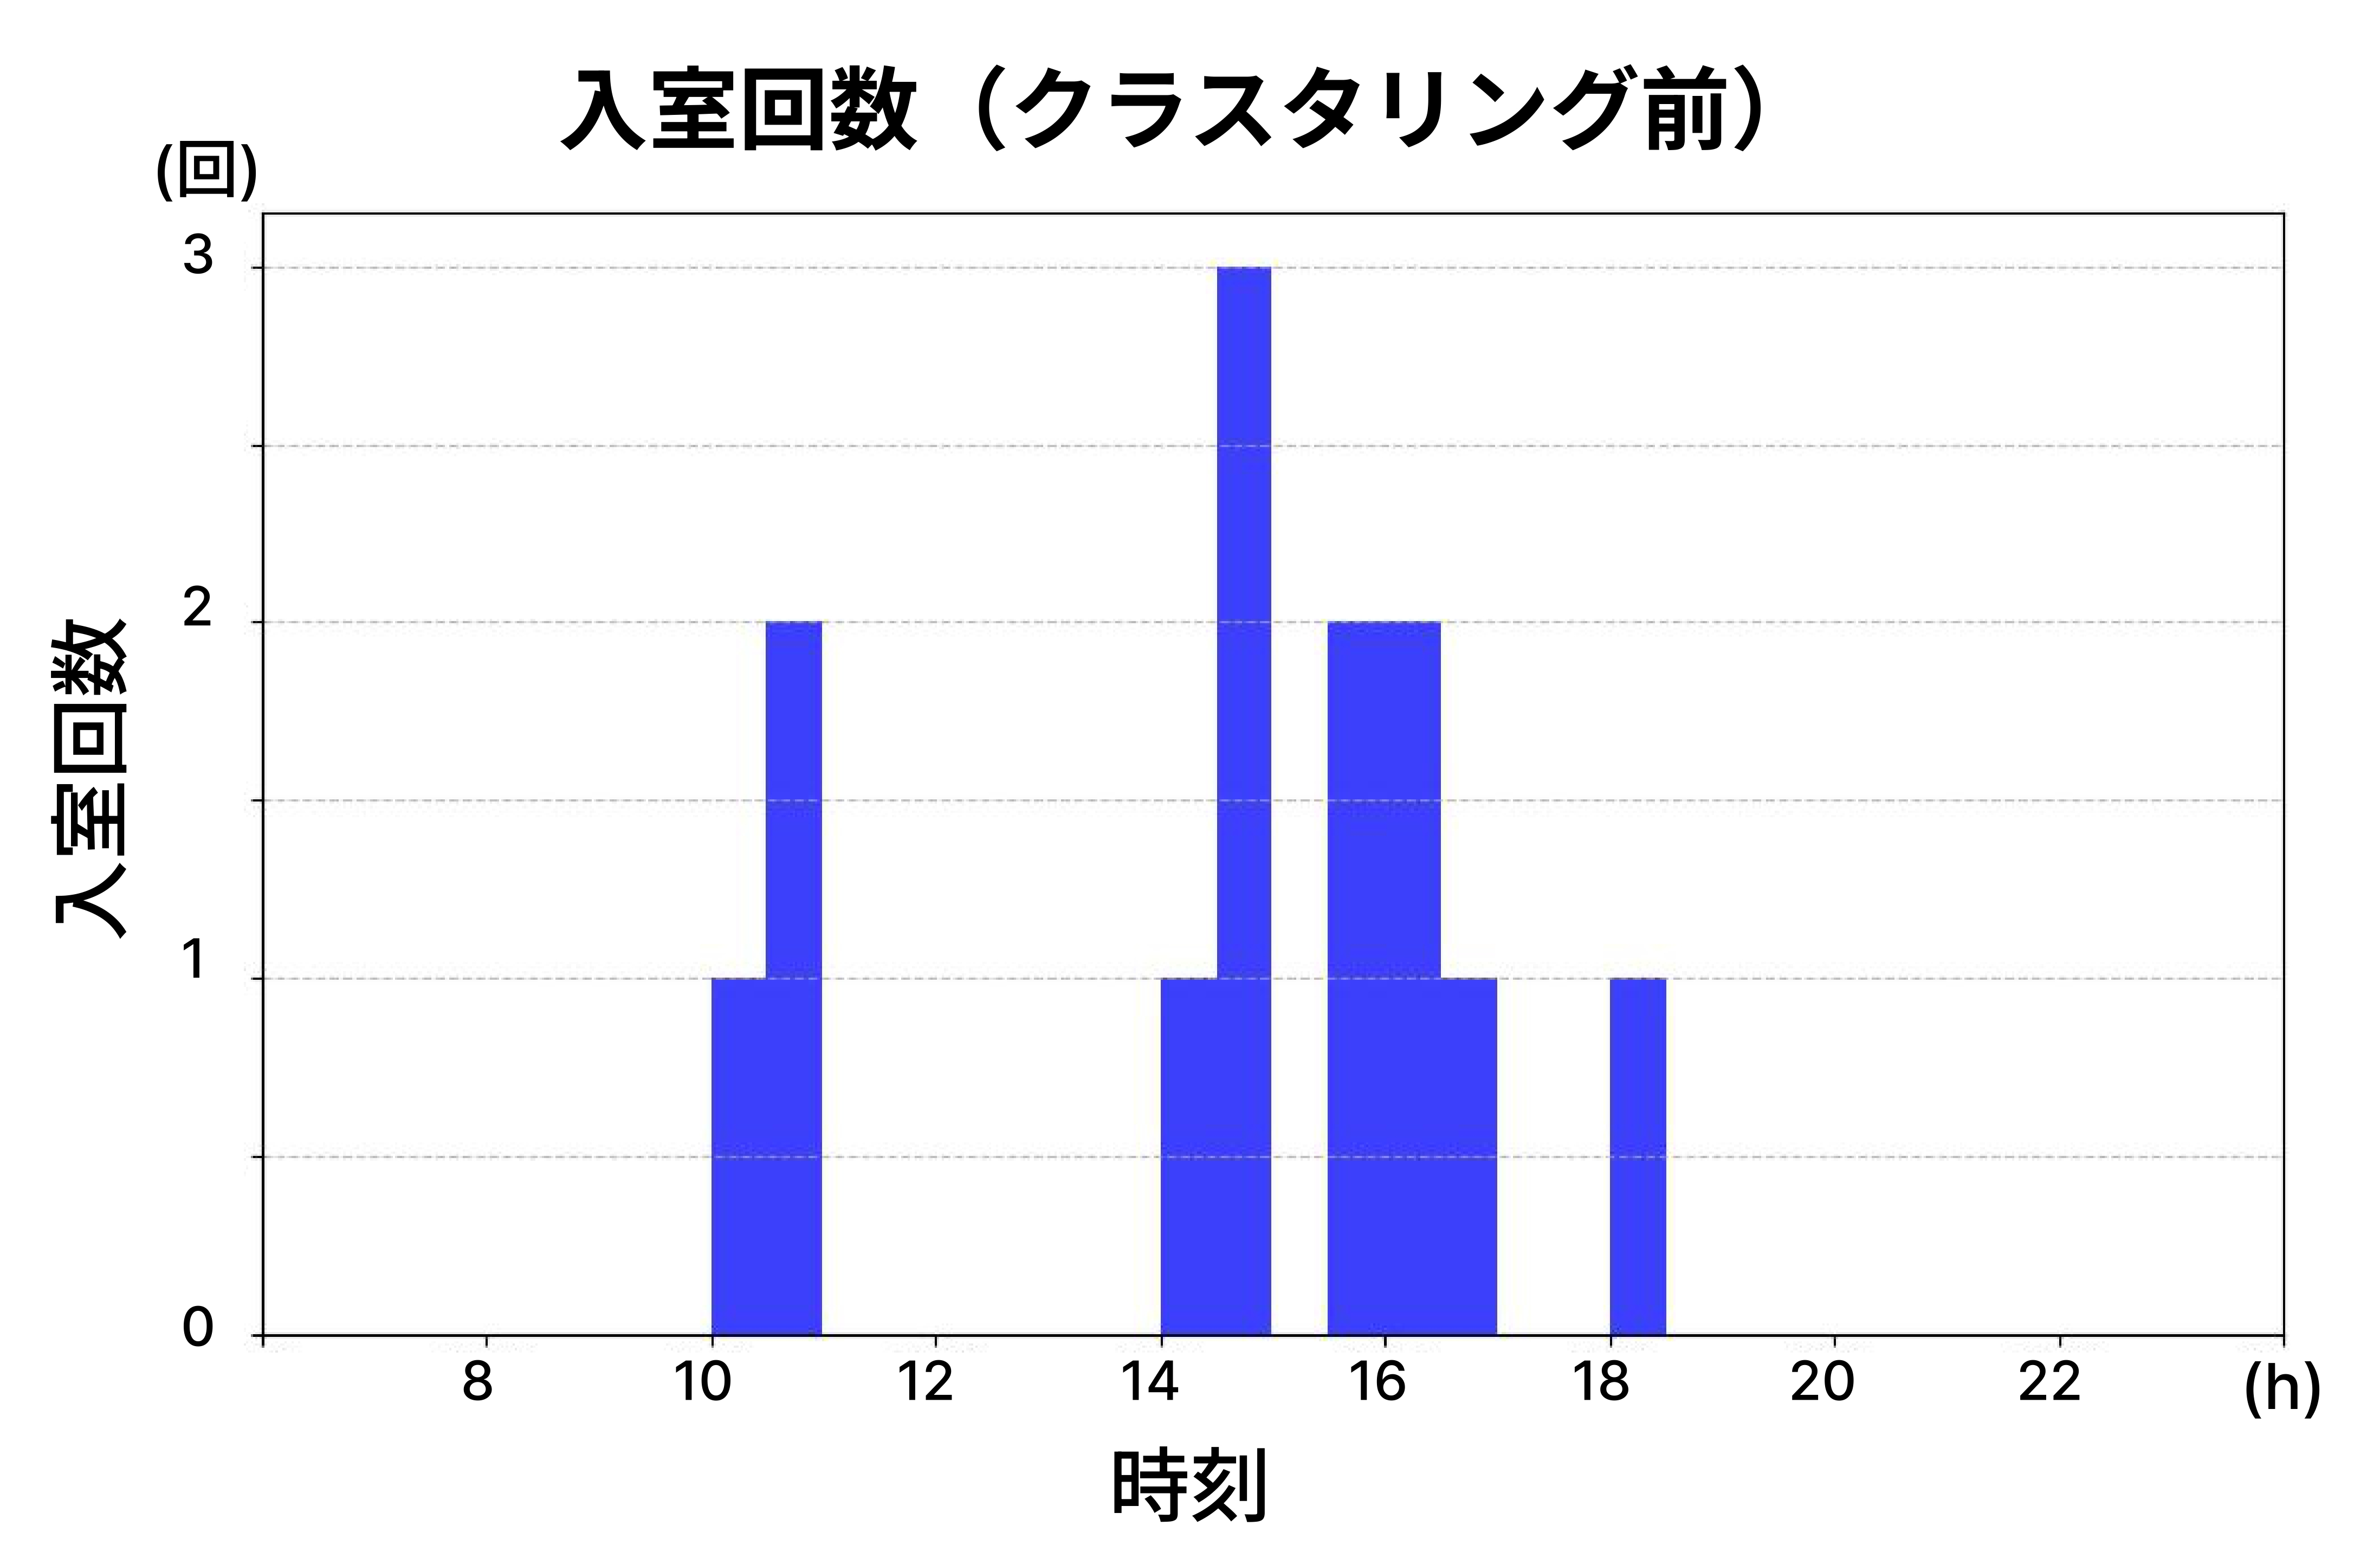
\includegraphics[width=0.45\linewidth]{fig/beforeClustering.jpg}}
  \hspace{3mm}
  \subcaptionbox{クラスタリング後\label{fig:aftClus}}{
    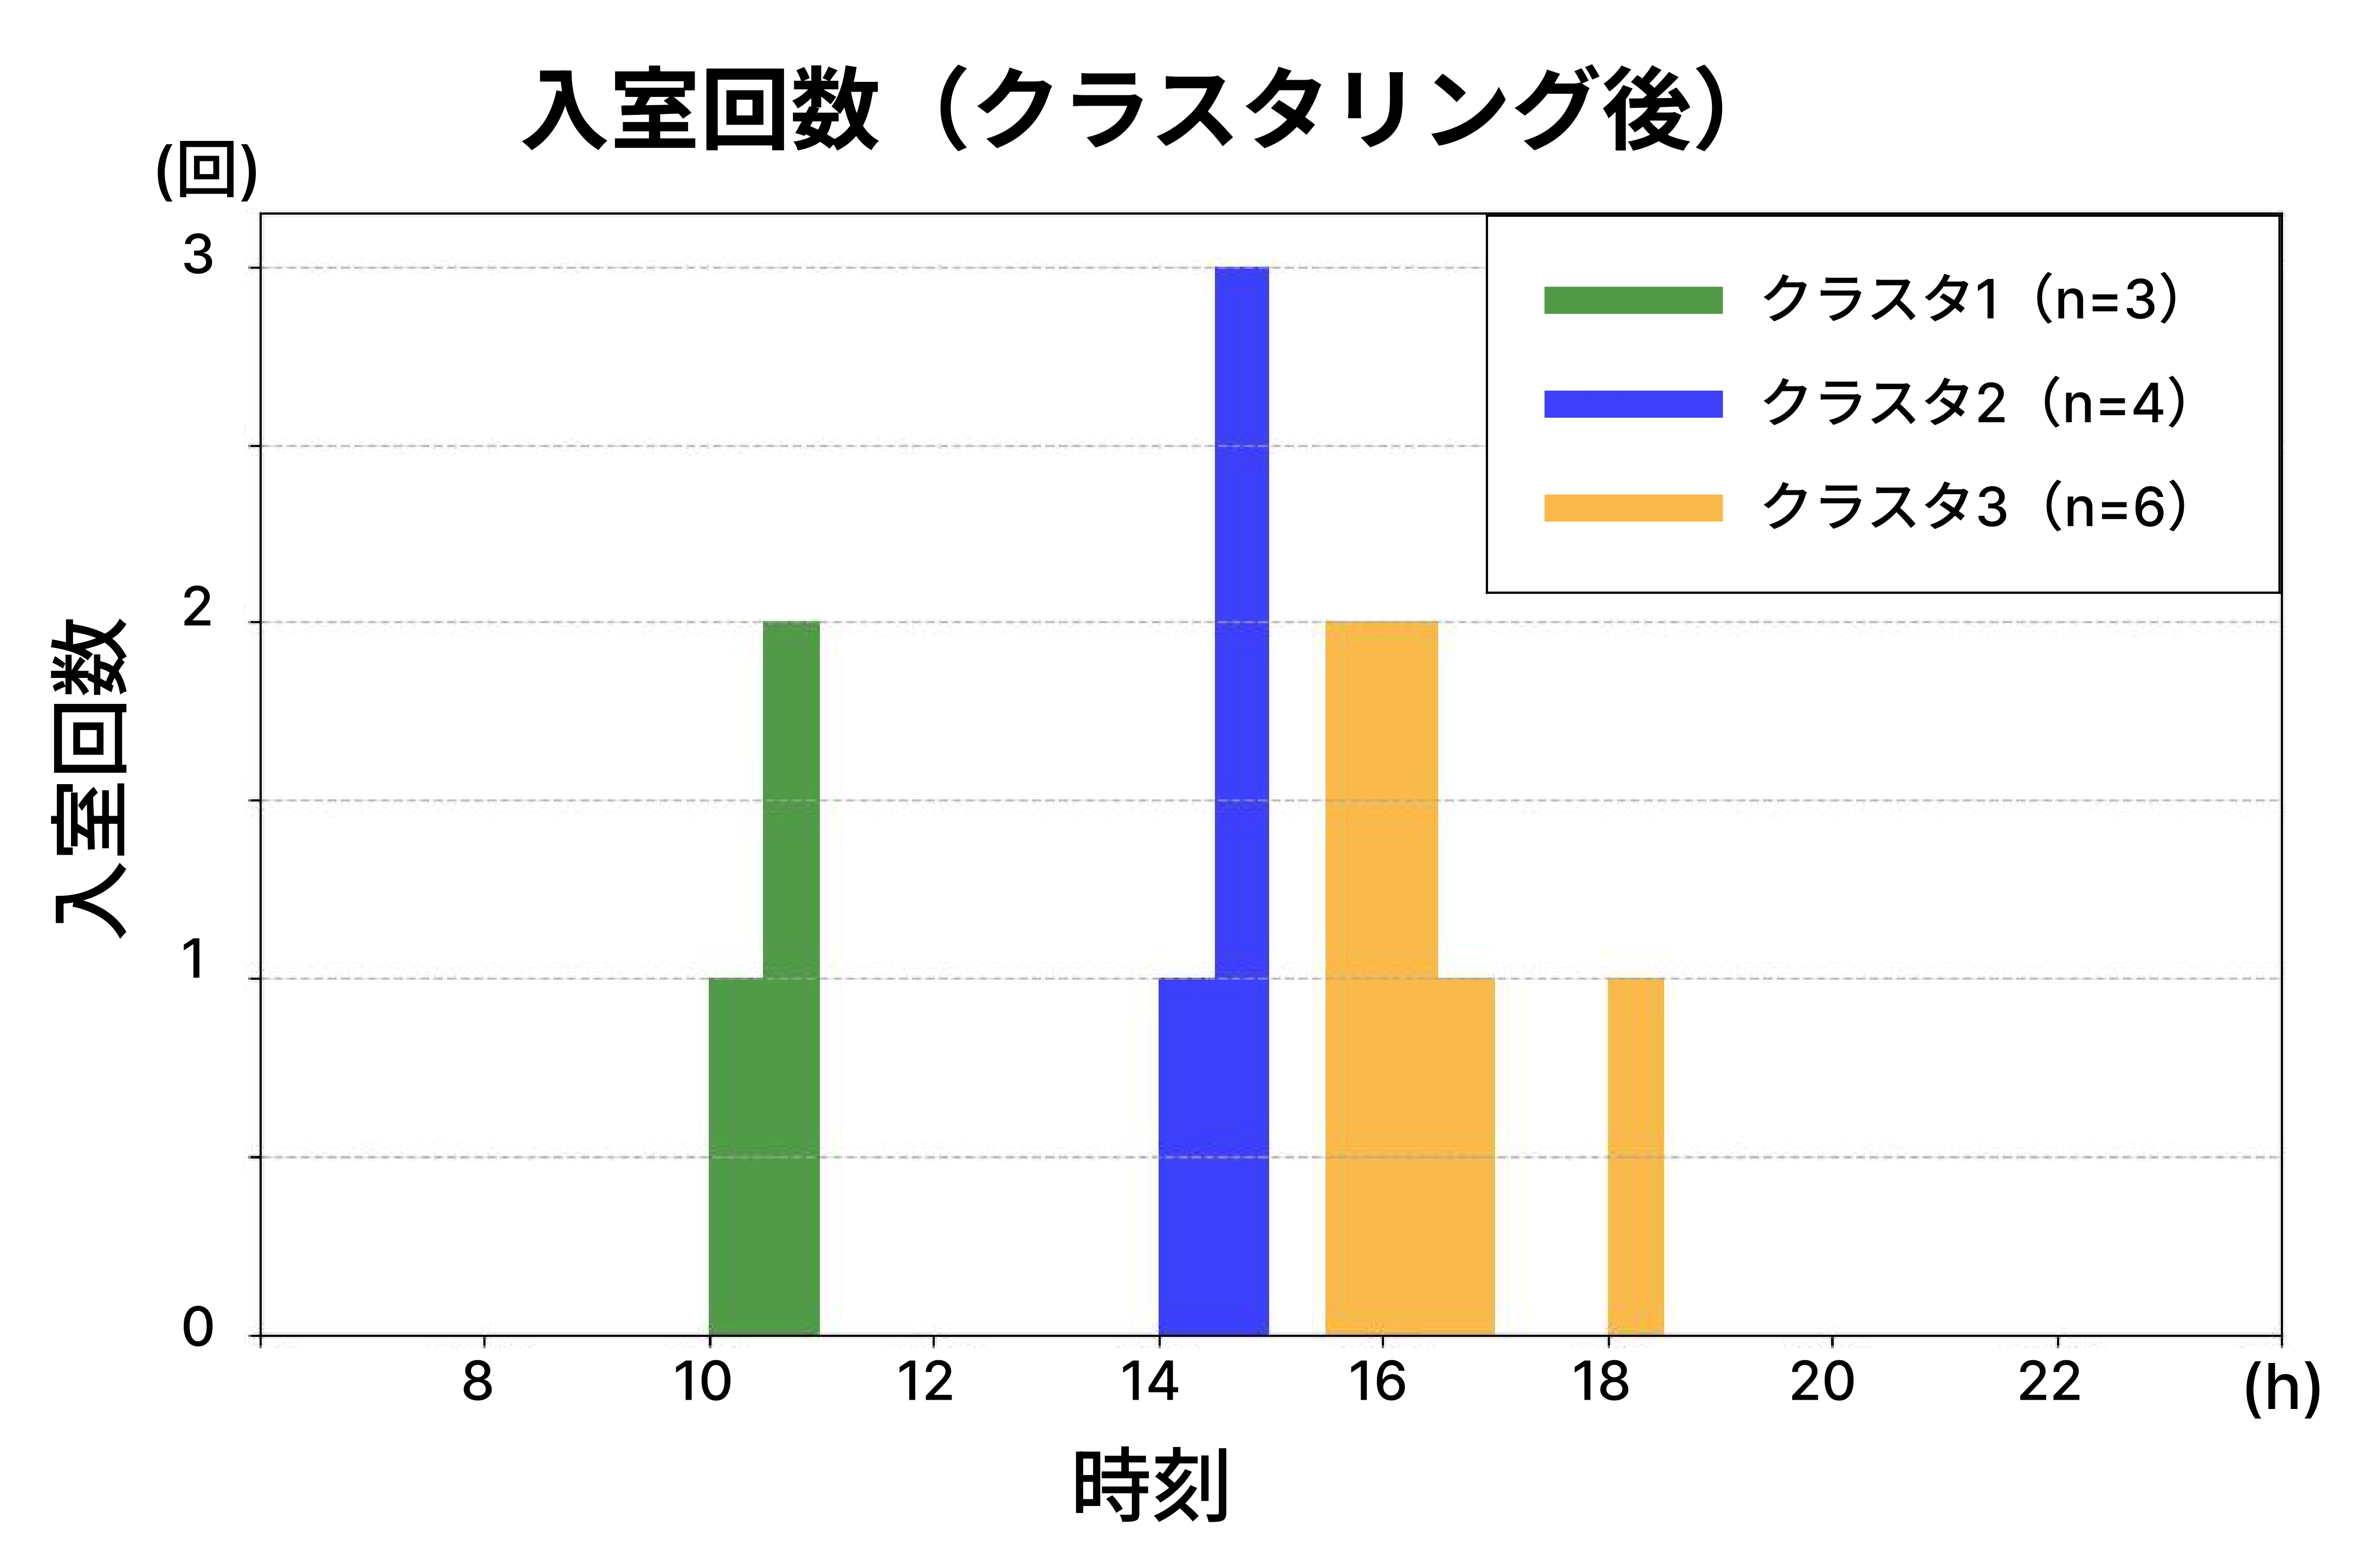
\includegraphics[width=0.45\linewidth]{fig/afterClustering.jpg}}
  \hspace{3mm}
  \subcaptionbox{累積分布関数（重み付け前）\label{fig:befWeig}}{
    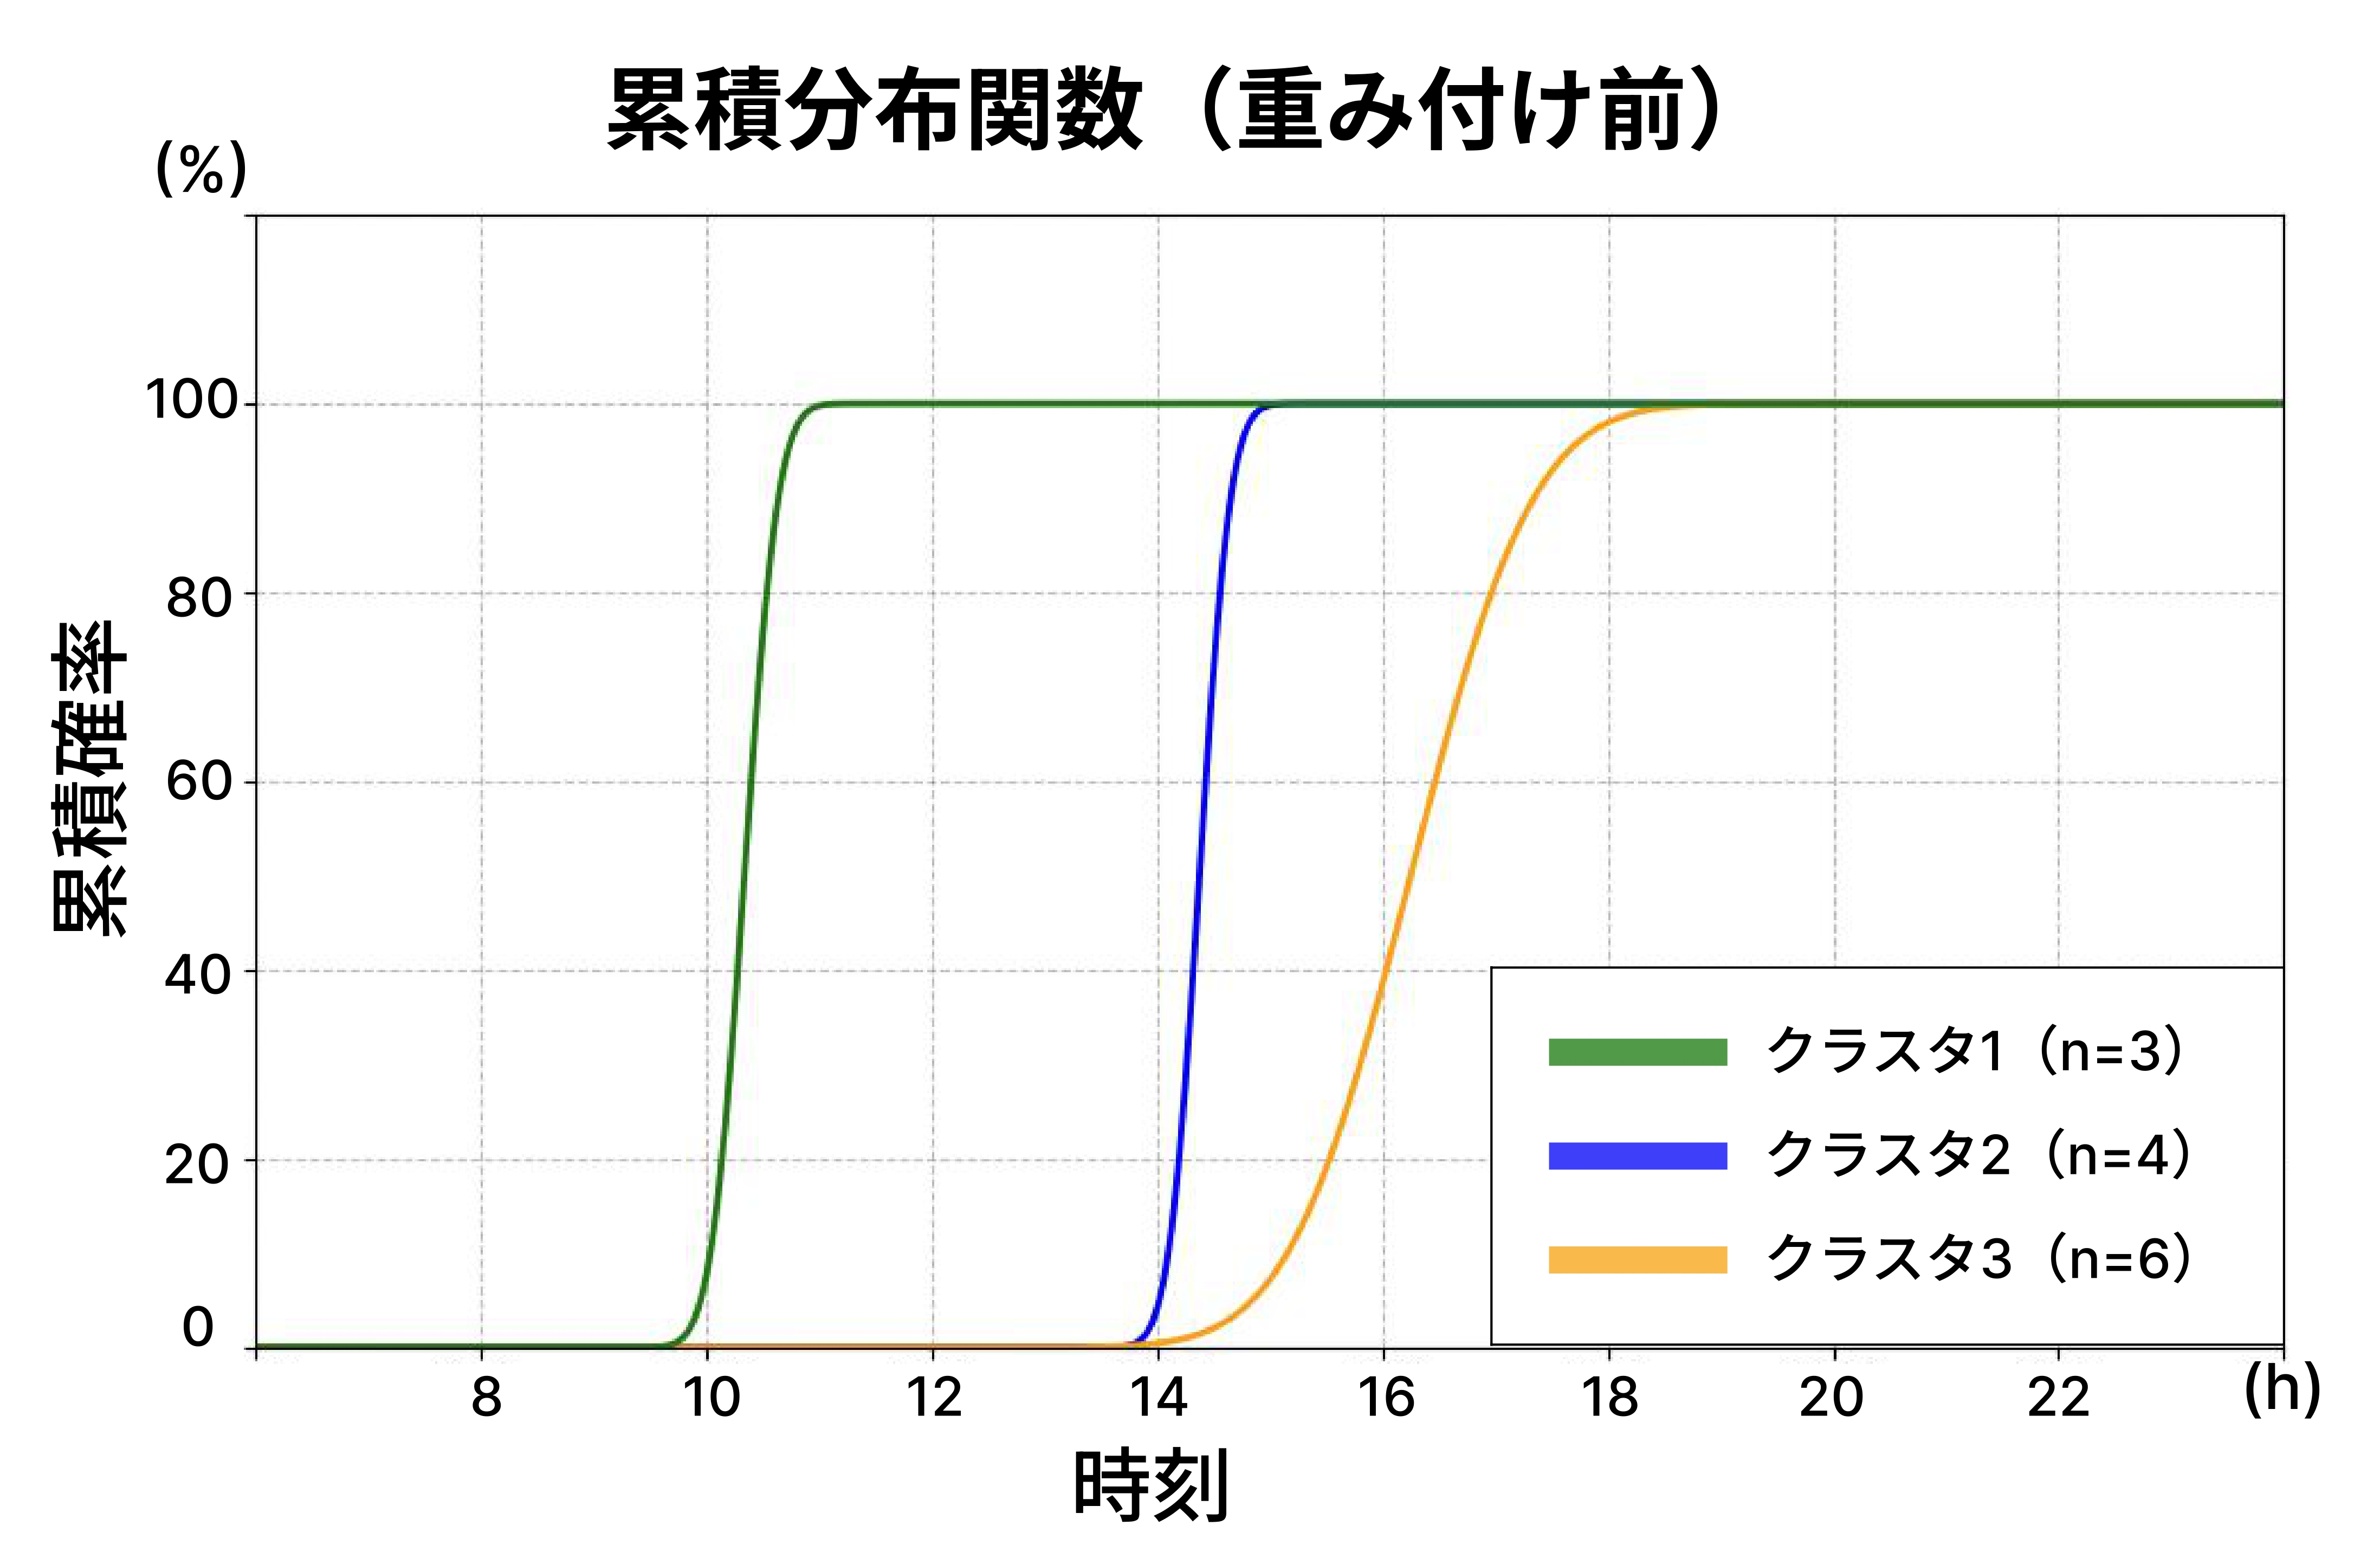
\includegraphics[width=0.45\linewidth]{fig/beforeWeighting.jpg}}
  \hspace{3mm}
  \subcaptionbox{累積分布関数（重み付け後）\label{fig:aftWeig}}{
    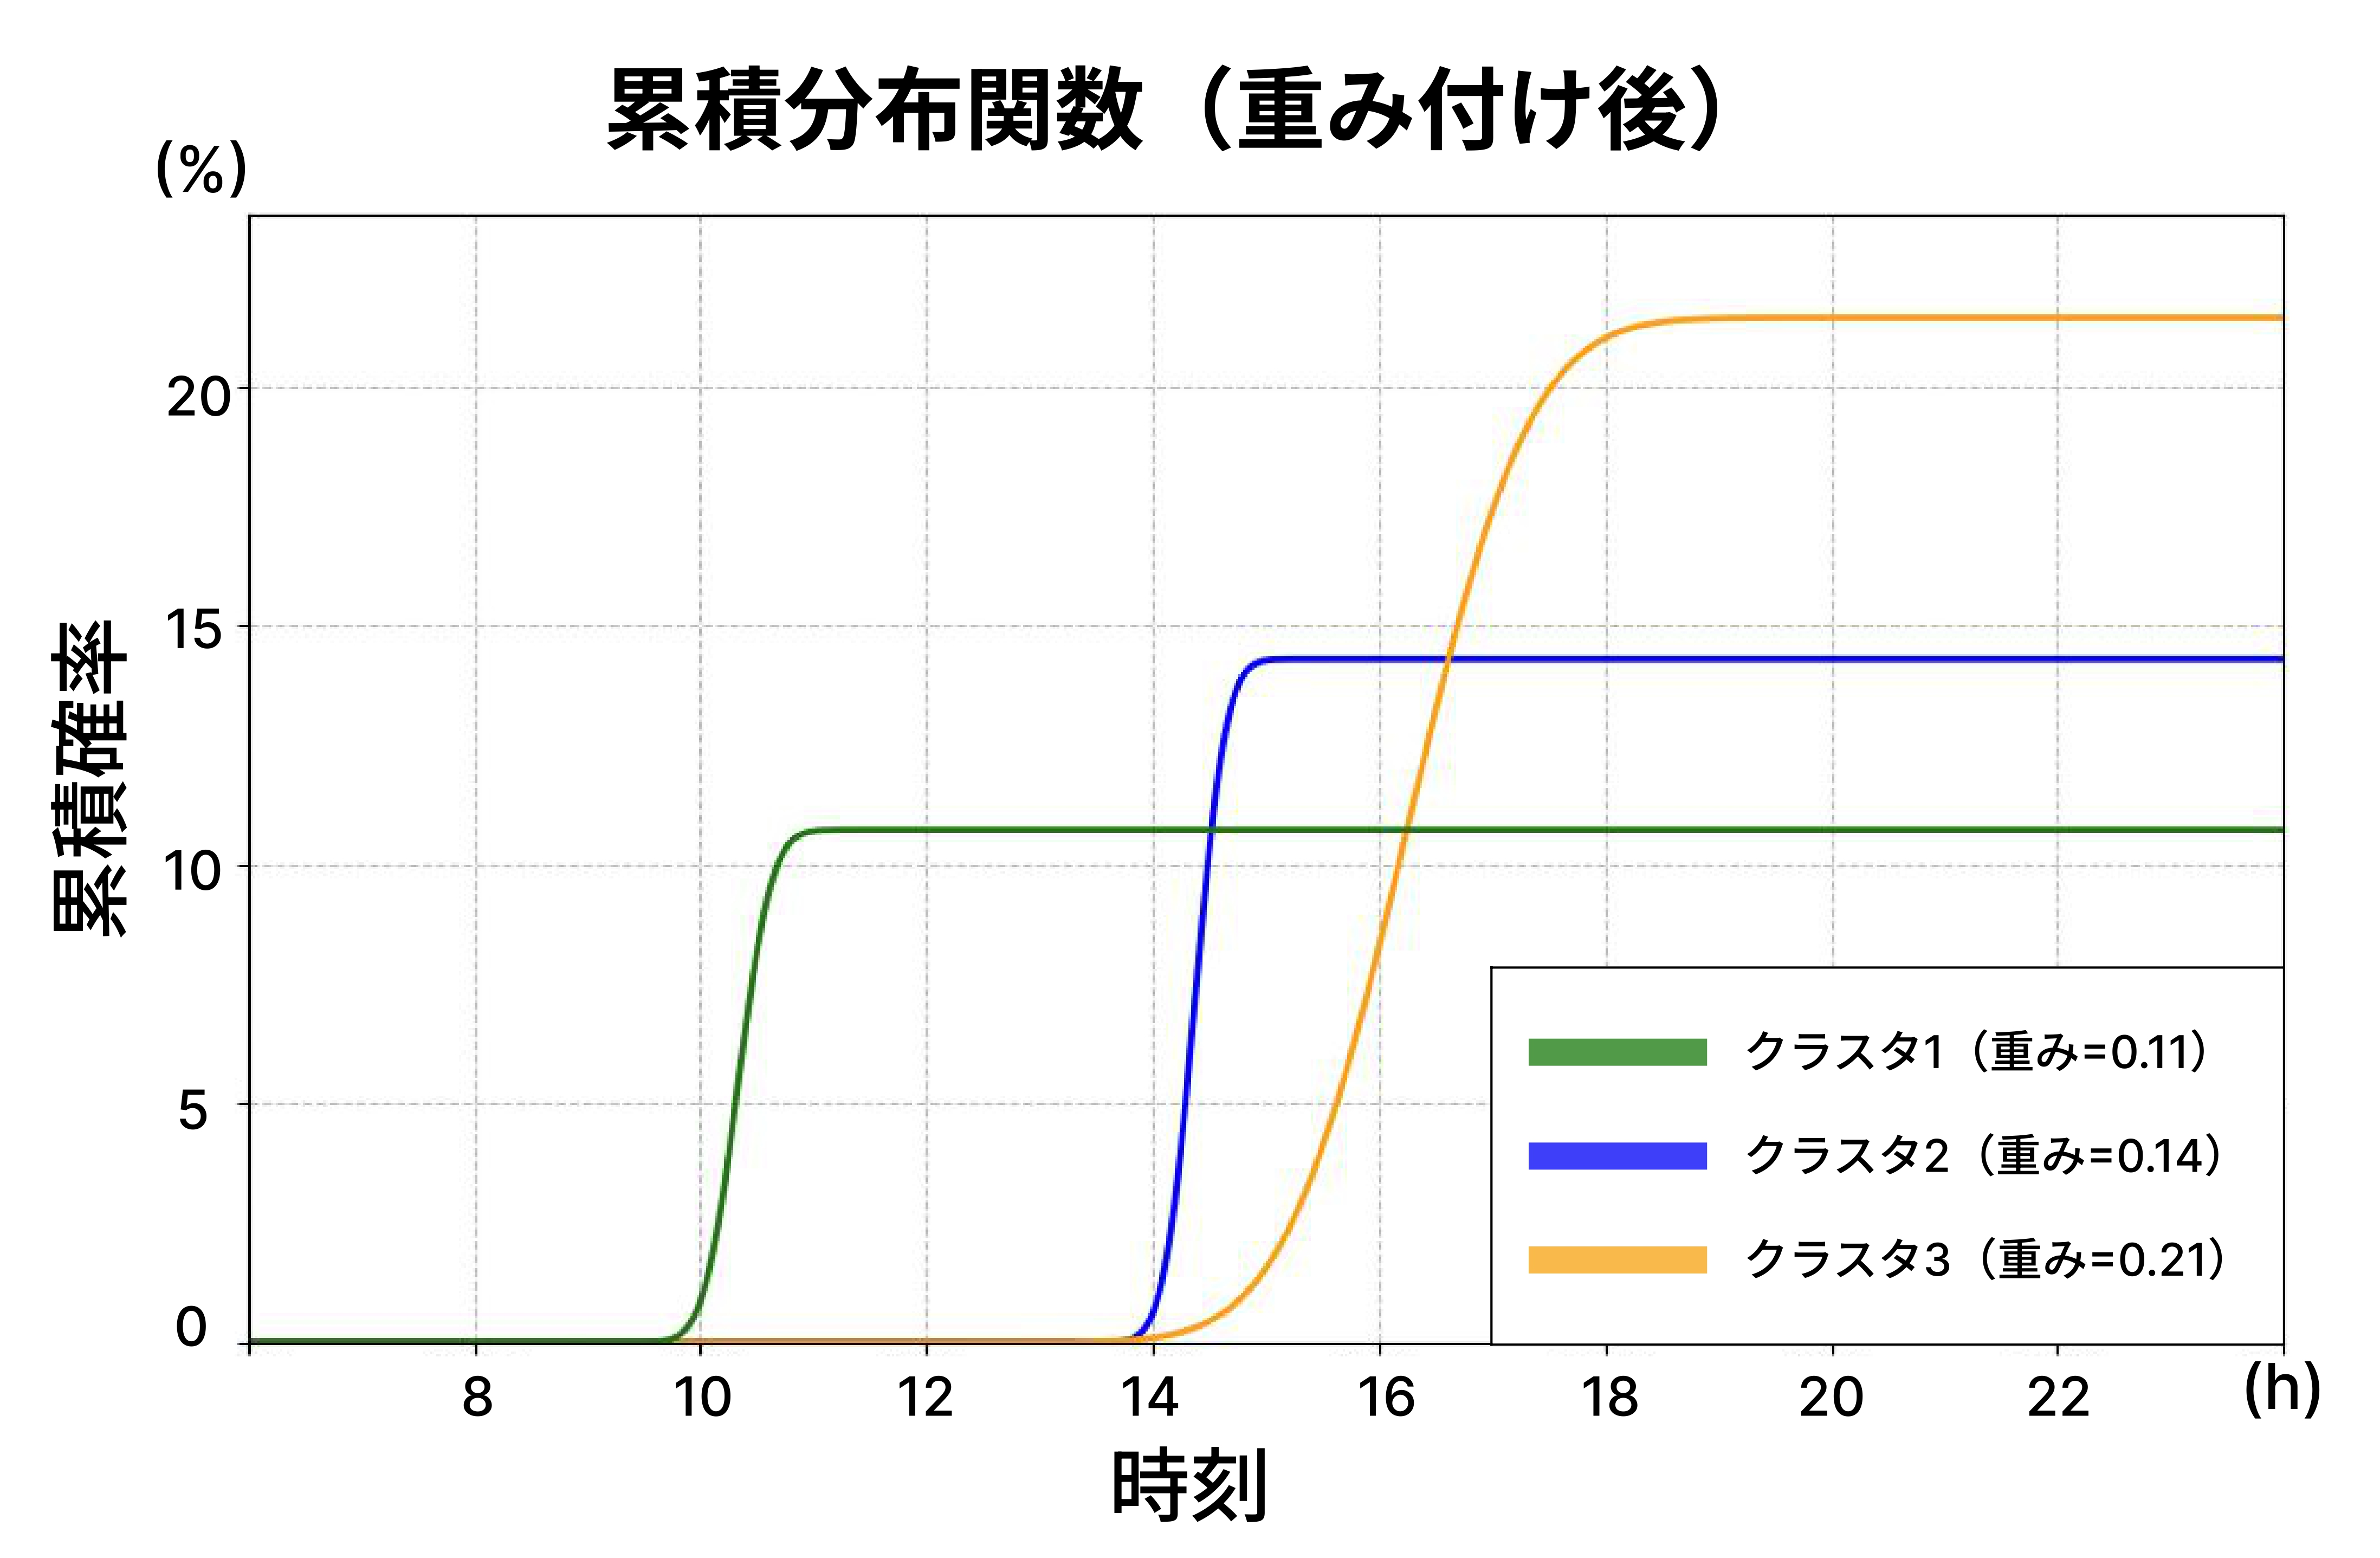
\includegraphics[width=0.45\linewidth]{fig/afterWeighting.jpg}}
  \hspace{3mm}
  \subcaptionbox{累積分布関数の合成\label{fig:synth}}{
    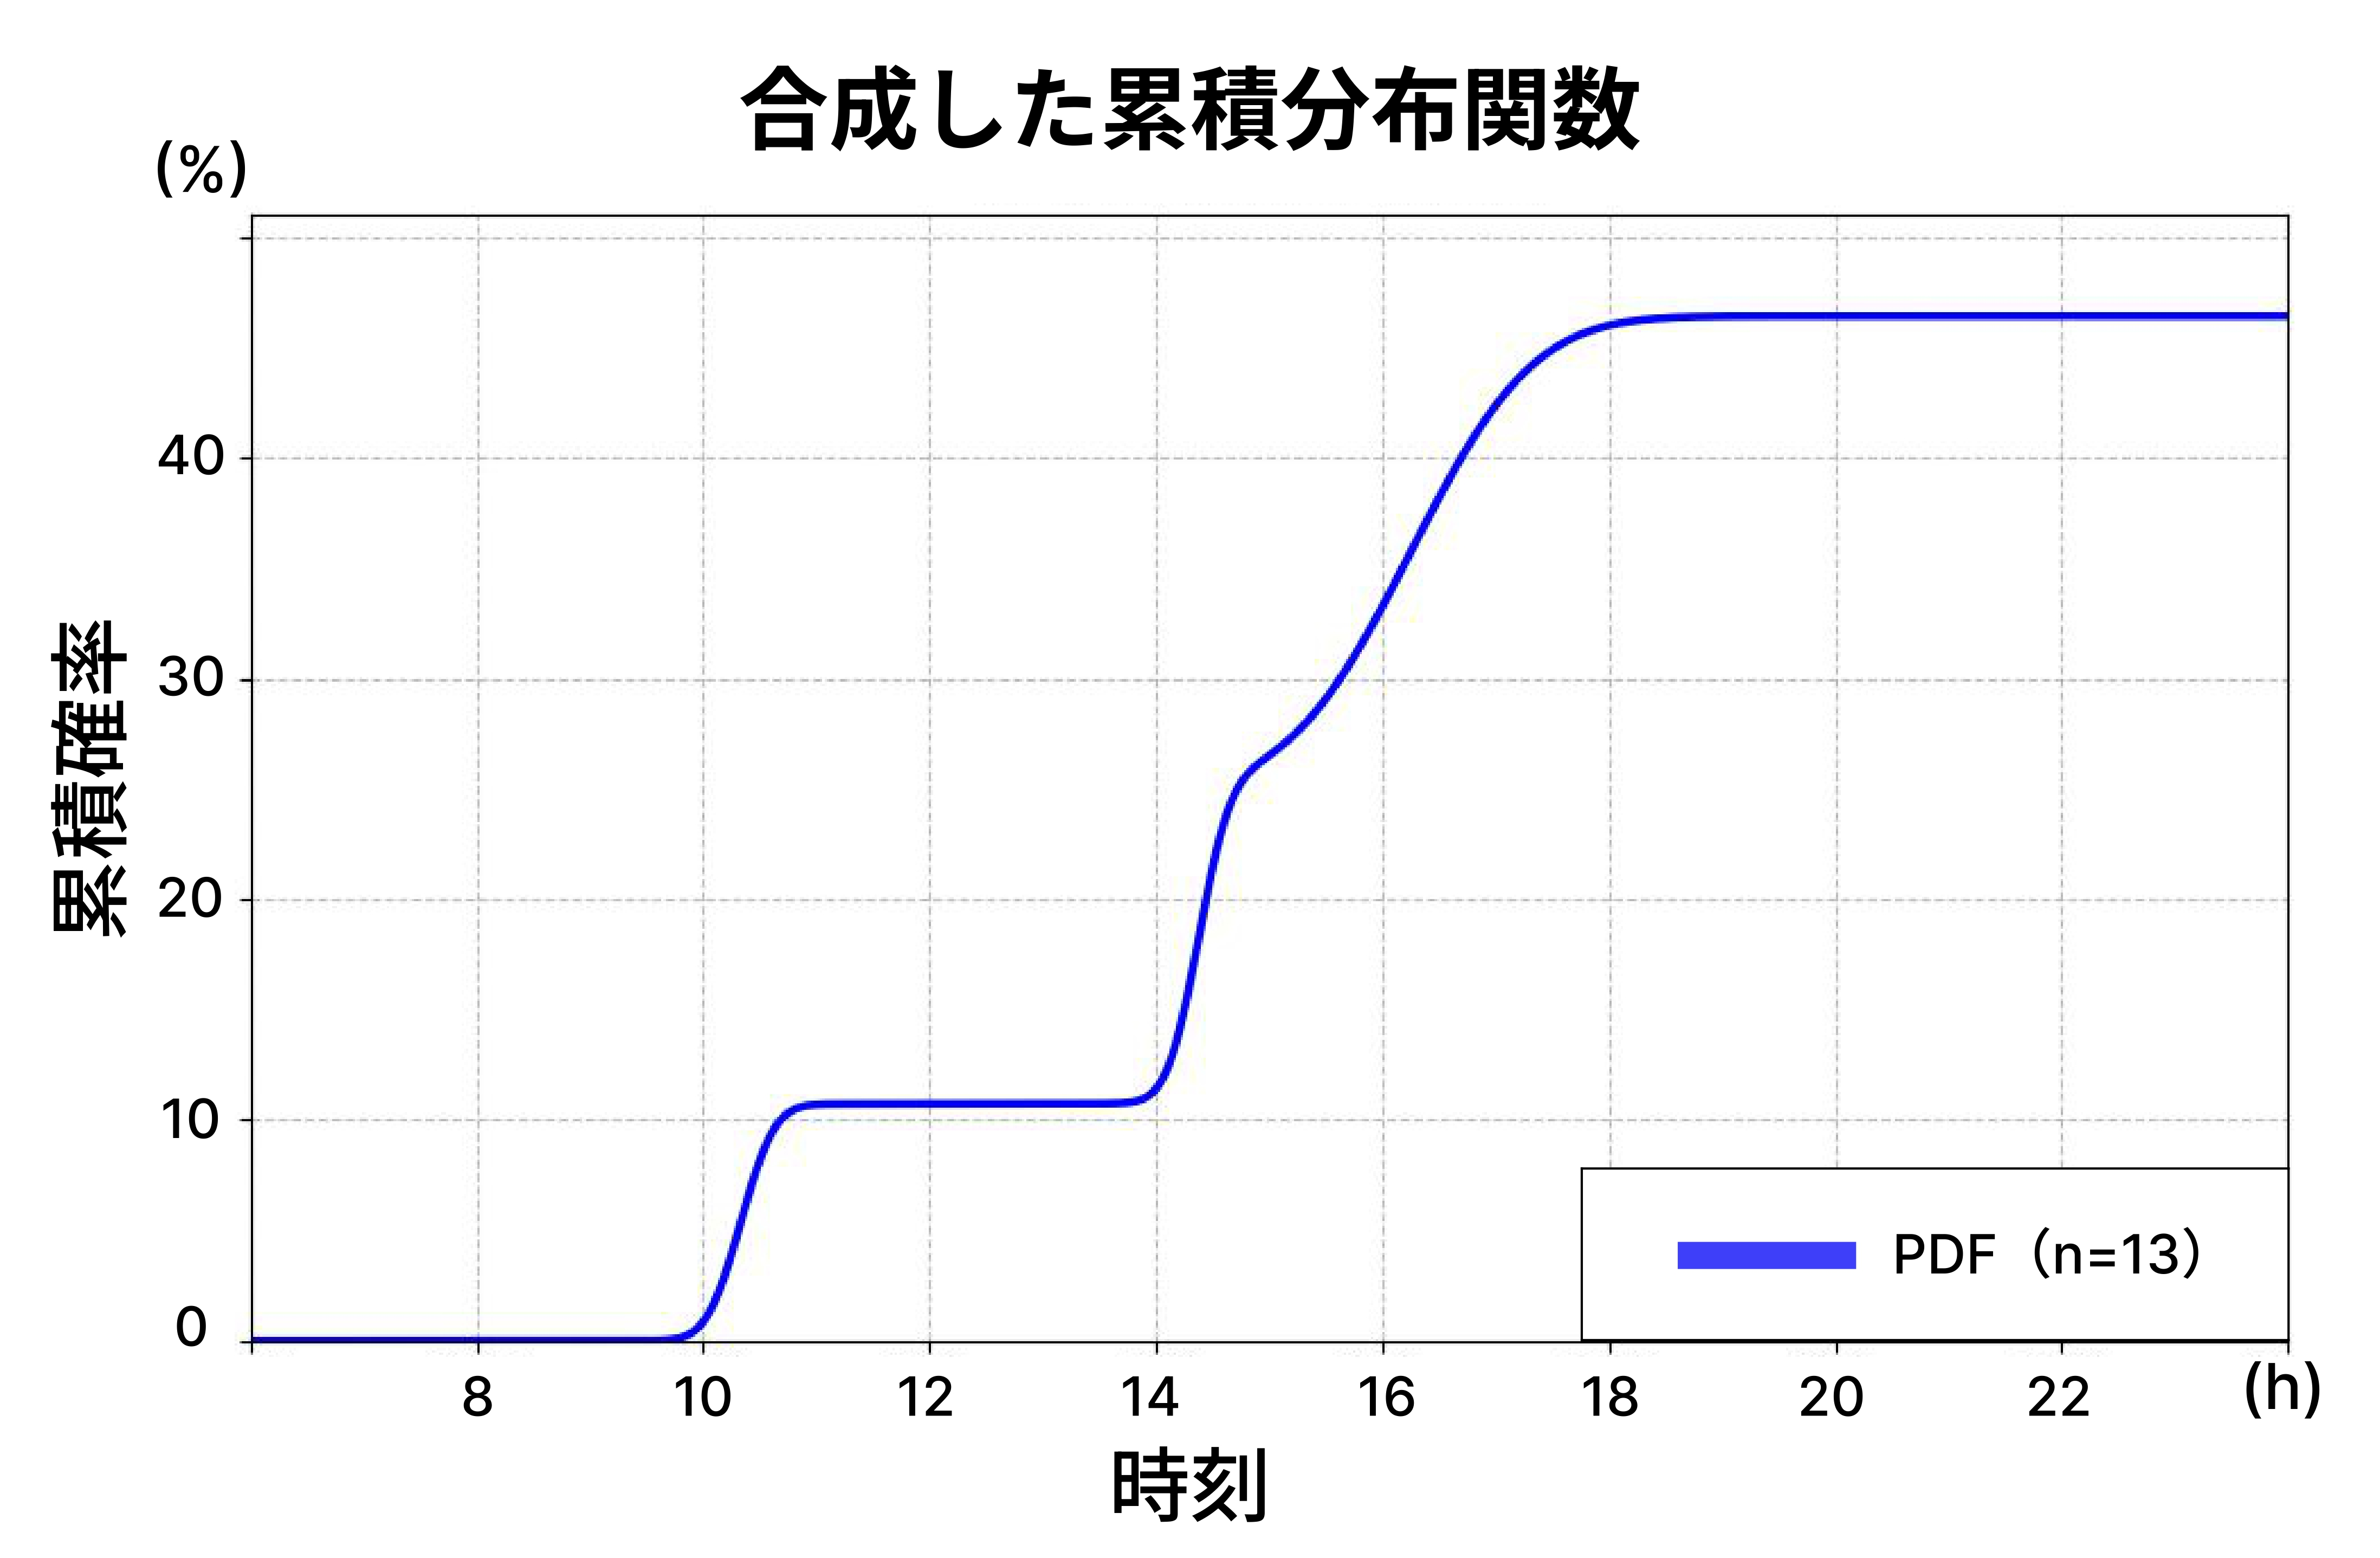
\includegraphics[width=0.45\linewidth]{fig/synthesis.jpg}}
  \caption{来訪確率の算出手順}
  \label{fig:prediction}
\end{figure}


% \paragraph{精度検証と考察}
% 実験設定も軽く
滞在ウォッチに記録されている大学生・大学院生32名の入退室履歴を用いて，「任意の時刻までに来訪している確率」が検証された．
具体的には，予測モデルにより算出された各曜日の合成された累積分布関数が，あらかじめ設定した閾値である50\%を超える時刻における予測確率と実際の来訪頻度が比較された．
全ユーザにおける検証結果が表\ref{tab:seido}である．
推定された確率値と実測値の平均値は概ね一致しており，大きな偏りなく来訪傾向を捉えていると確認されている．
一方，個人・曜日ごとに予測のばらつきが見られ，履歴の少なさや年末年始などの行動パターンの変化が考察されている．

\begin{table}[htb]
  \centering
  \caption{来訪確率予測の全体集計結果(文献\cite{hayashi}より引用)}
  \label{tab:seido}
  \begin{tabular}{|l|l|}
    \hline
    \textbf{項目} & \textbf{値} \\
    \hline
    平均予測確率      & 50.16\%    \\
    平均実測値       & 49.77％     \\
    平均誤差        & 0.39 ポイント  \\
    平均絶対誤差      & 18.29 ポイント \\
    平均絶対誤差率     & 0.646      \\
    \hline
  \end{tabular}
\end{table}